\section{روش پیاده‌سازی}\label{sec:implementation}

\subsection{مقدمه}\label{subsec:impl_intro}
برای پیاده‌سازی یک سامانه، می‌توان دو رویکرد داشت. می‌توان از سامانه‌های از پیش موجود استفاده کرد و با حاصل کردن تغییرات لازم به مقصود رسید. و یا می‌توان با پیاده‌سازی سامانه از ابتدا، نیاز‌های را حل کرد.

از طرفی با توجه به ویژگی‌های ذکرشده در فصل
\ref{sec:sources}
، راه حل انتخابی برای پیاده‌سازی یک درگاه ارتباط با رابط‌های برنامه‌نویسی باید معیار‌های زیر را مدنظر خود قرار داده باشد:

\begin{itemize}
    \item سرعت بالا
    \item کارایی بالا
    \item بهینه‌بودن راه‌حل
    \item گسترش‌پذیری
    \item تغییر‌پذیری
    \item سادگی و قابل فهم بودن
\end{itemize}

\subsection{انتخاب روش و فناوری}\label{subsec:impl_choose}
استفاده‌ از فناوری‌های موجود، مانند \lr{Nginx}، \lr{HAProxy} و ... و ایجاد تغییرات در آن‌ها جهت بر طرف کردن نیاز‌های مطرح شده در فصل
\ref{sec:sources}
، می‌تواند یکی از راه‌حل ‌های حل مسئله باشد. ولی با توجه به پایه‌ی پیاده‌سازی این محصولات بر اساس نیاز‌های گذشته، و همچنین عدم سازگاری این محصولات با محیط‌های ابری، جهت استفاده به عنوان درگاه ارتباط با رابط‌های برنامه‌نویسی، مشکلات زیادی برای حل مسئله وجود خواهد آمد. برخی از این مشکلات عبارتند از:

\begin{itemize}
    \item اجبار به استفاده از راه‌حل‌های موقتی برای سازگاری این محصولات با فضای موجود
    \item پیچیدگی بیش از حد به دلیل وجود ویژگی‌های مرتبط با حوزه‌های دیگر
    \item احتمال عدم سازگاری تغییرات مورد نظر با ویژگی‌های اصلی محصول
    \item و \ldots
\end{itemize}

از این رو پیاده‌سازی یک درگاه، از ابتدا و با توجه به نیاز‌های جدید،‌ راه حل منطقی تری به نظر می‌رسد.

با توجه به نیاز سامانه‌ به دسترسی‌های سطح پایین، جهت ارتباط با لایه‌ی هفتم شبکه، و همچنین نیاز به سرعت بالا برای کنترل بار، زبان‌های برنامه‌نویسی محدودی مناسب پیاده‌سازی این محصول خوا‌هند بود. برخی از این گزینه‌ها عبارتند از:

\begin{itemize}
    \item زبان برنامه‌نویسی کامپایلری C/C++
    \item زبان برنامه‌نویسی کامپایلری Golang
    \item زبان برنامه‌نویسی مفسری Lua
    \item زبان برنامه‌نویسی Javascript (بستر \lr{Node.js})
\end{itemize}

معمولا زبان‌های برنامه‌نویسی سطح پایین‌تر، سرعت بالاتری نیز دارند. از این رو زبان‌های C و C++ از بالاترین سرعت برخوردار هستند. با این وجود، کاری‌هایی مانند مدیریت حافظه، مدیریت پردازه‌های هم‌روند و ... به عهده‌ی برنامه‌نویس است. این امر باعث پیچیدگی توسعه خواهد بود. از این رو، زبان برنامه‌نویسی Golang، که یک زبان برنامه‌نوسی سطح‌ پایین محسوب می‌شود، به علت مدیریت حافظه خودکار و استفاده‌ی ساده از پردازه‌ها
\LTRfootnote{Process}
و ریسمان‌ها
\LTRfootnote{Thread}
برای اجرای فرآیند‌های هم‌روند، می‌تواند گزینه‌ی مناسبی جهت پیاده‌سازی باشد.

از زبان‌های مفسری نیز می‌توان برای توسعه‌ی نرم‌افزار‌هایی که در زمان اجرا نیاز به تغییر در خود دارند، استفاده کرد. ولی نقطه‌ی تاریک استفاده ‌از زبان‌های برنامه‌نویسی مفسری، احتمال بالای رخداد خطا‌های زمان اجرا خواهد بود. این ویژگی باعث از دست رفتن ثبات سامانه می‌شود.

نحوه‌ی انجام فرآیند‌های هم‌روند نیز در انتخاب فناوری پیاده‌سازی این بخش از سامانه بسیار تاثیرگذار است. زیرا با توجه به نیاز به توان عملیاتی بالا، فناوری‌های تک رشته‌ای و یا تک‌ پردازه‌ای باعث کاهش توان عملیاتی سامانه خواهند شد.

جدول
\ref{tab:choice}
شامل مقایسه‌ی زبان‌های برنامه‌نویسی ذکر شده با توجه‌ به معیار‌های ذکر شده است.

\begin{table}[H]
    \centering
    \caption{مقایسه‌ی زبان‌های برنامه‌نویسی جهت پیاده‌سازی درگاه ارتباط با رابط‌های برنامه‌نویسی}\label{tab:choice}
    \begin{tabular}{|c|c|c|c|c|c|c|}
        \hline
        زبان برنامه‌نویسی & سرعت & سادگی & بهینگی & توان عملیاتی & مدیریت حافظه & مدیریت فرآیند‌های هم‌روند\\
        \hline
        C/C++ & بسیار بالا & پایین & بسیار بالا & بسیار بالا & خیر & بسیار سخت\\
        \hline
        Golang & بالا & متوسط & بالا & بالا & بله & آسان\\
        \hline
        Lua & بالا & متوسط & بالا & متوسط & بله & سخت\\
        \hline
        Javascript & متوسط & بالا & پایین & متوسط & بله & سخت\\
        \hline
    \end{tabular}

\end{table}


با توجه به جدول
\ref{tab:choice}
، روش انتخابی برای حل مسئله،‌ پیاده‌سازی سامانه از ابتدا و با استفاده از زبان برنامه‌نویسی Golang است. زیرا با اینکه سرعت کمتری نسبت به زبان برنامه‌نویسی C یا C++ دارد، ولی با توجه به عدم نیاز به مدیریت حافظه، مدیریت آسان‌تر فرآیند‌های هم‌روند و همچنین سادگی و بهینگی قابل قبول،‌ می‌توان از اختلاف سرعت این دو زبان برنامه‌نویسی چشم پوشی کرد.

\subsection{پیاده‌سازی}\label{subsec:impl_impl}

\subsubsection{ساختار}
ساختار برنامه‌ باید به شکلی تعیین شود که برنامه‌نویس را در روند توسعه برنامه محدود نکند. علاوه بر این، یک ساختار خوب می‌تواند زمینه را جهت معماری گسترش‌پذیر و منعطف فراهم کند.

یکی از ساختار‌های مناسب، در محیط توسعه‌ی Golang ، ساختار بسته مبنا است. این ساختار توسط بسیاری از محصولات صنعتی و آکادمیک استفاده شده است. همچنین برخی از ابزار‌های از پیش‌آماده در محیط توسعه‌ی این زبان، از سازگاری کامل با این ساختار برخوردار هستند.

\subsubsection{ساختار بسته‌مبنا \LTRfootnote{Package Oriented}}
این ساختار، شامل سه پوشه‌ی اصلی \lr{cmd}، \lr{internal} و \lr{pkg} است. پوشه‌های config و logging از جمله پوشه‌های دیگر این ساختار هستند که استفاده از آن‌ها توصیه شده است.

پوشه‌ی cmd حاوی برنامه‌ی اصلی و قابل اجرا است. این پوشه معمولا دارای برنامه‌های کوتاه و با منطق ساده هستند.

پوشه‌ی pkg حاوی بسته‌های مستقل و قابل استفاده توسط سایر برنامه هاست. بسته‌های موجود در این پوشه به تنهایی قابل استفاده اند و وابستگی آن‌ها به دیگر بسته ها بسیار کم است.

پوشه‌ی internal دارای بسته‌هایی است که از بسته‌های موجود در pkg استفاده کرده و منطق اصلی برنامه را پیاده‌سازی می‌کند. در این پوشه، رابط‌های ورودی و خروجی برنامه تعیین می‌شود.

بسته‌ی logging شامل برنامه‌های مربوط به ثبت اتفاقات سامانه است.

بسته‌ی config نیز دربردارنده‌ی برنامه‌های مربوط به پیکربندی و تنظیمات اجرای برنامه است. نحوه‌ی بارگذاری پیکربندی‌ها و همچنین استفاده از تنظیمات در قسمت‌های مختلف برنامه در این قسمت پیاده‌سازی می‌شود.

نمونه‌ی یک ساختار بسته‌مبنا در شکل
\ref{package_oriented}
قابل مشاهده است.

\begin{figure}[H]
    \centering
    \caption{نمونه‌ی یک ساختار بسته مبنا}
    \label{package_oriented}
    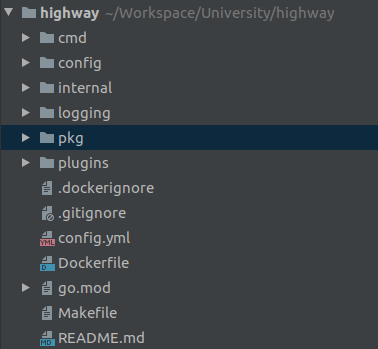
\includegraphics[scale=0.4]{images/PackageOriented.png}
\end{figure}

\cleardoublepage

\subsection{مفاهیم}\label{subsec:impl_concepts}
برای پیاده‌سازی یک درگاه ارتباط با رابط‌های برنامه‌نویسی، مفاهیم زیر پیشنهاد شده است:

\begin{itemize}
    \item بطن \LTRfootnote{Backend}
    \item خدمت \LTRfootnote{Service}
    \item متعادل‌کننده‌ی بار \LTRfootnote{Load Balancer}
    \item ضابطه \LTRfootnote{Rule}
    \item میان‌افزار \LTRfootnote{Middleware}
    \item مسیریاب \LTRfootnote{Router}
    \item تامین کننده‌ی خدمت \LTRfootnote{Service Provider}
\end{itemize}

در ادامه به توضیح هر یک از مفاهیم ذکر‌ شده پرداخته‌ می‌شود.

\subsubsection{بطن}
یک بطن، کوچک‌ترین واحد در این سامانه است. هر بطن، یک داده ساختار شامل نام، آدرس، وزن و وضعیت است. این چهار ویژگی نشان‌دهنده‌ی یک نمونه از رابط‌های برنامه‌نویسی قابل استفاده توسط برنامه است. داده‌ساختار زیر، نشان‌دهنده‌ی بطن است.

\begin{latin}
    \begin{lstlisting}
                                    type Backend struct {
                                        Name string
                                        Addr string
                                        Weight int8
                                        Status int
                                    }
    \end{lstlisting}
\end{latin}


\subsubsection{خدمت}
یک خدمت دارای یک نام، چند بطن و یک متعادل‌کننده‌ی توزیع بار است. معمولا بطن‌های یک خدمت کاملا مشابه یکدیگر عمل می‌کنند. با توجه به قسمت
\ref{subsubsec:impl_loadbalancer}
، خدمت با استفاده از متعادل‌کننده‌ی بار درخواست‌های را بین بطن‌های خود توزیع می‌کند.

قطعه کد زیر نشان‌دهنده‌ی داده‌ساختار یک خدمت است.

\begin{latin}
    \begin{lstlisting}
                                    type Service struct {
                                        Name     string
                                        Backends []Backend
                                        LB       LoadBalancer
                                    }
    \end{lstlisting}
\end{latin}

\subsubsection{متعادل‌کننده‌ی بار}\label{subsubsec:impl_loadbalancer}
این موجودیت در برنامه از نوع یک واسط
\LTRfootnote{Interface}
است. این واسط بدون در نظر گرفتن منطق پیاده‌سازی توزیع بار، رفتار‌های مورد نیاز برای این عمل را مشخص می‌کند.

این واسط به طور مستقیم قابل استفاده نیست. بلکه نسخه‌های پیاده‌سازی شده‌ی این واسط را می‌توان به طور مستقیم استفاده کرد. برای مثال، الگوریتم توزیع تصادفی جهت توزیع بار در این برنامه پیاده‌سازی شده است. برنامه‌ی زیر نشان‌دهنده‌ی واسط متعادل‌کننده‌ی بار و شکل
\ref{service_package}
حاوی نمودار پیاده‌سازی نمونه‌ها از واسط هستند.


\begin{latin}
    \begin{lstlisting}
                                    type LoadBalancer interface {
                                        Balance([]Backend) Backend
                                    }
    \end{lstlisting}
\end{latin}


\begin{figure}[H]
    \centering
    \caption{نمودار UML بسته‌ی Service}
    \label{service_package}
    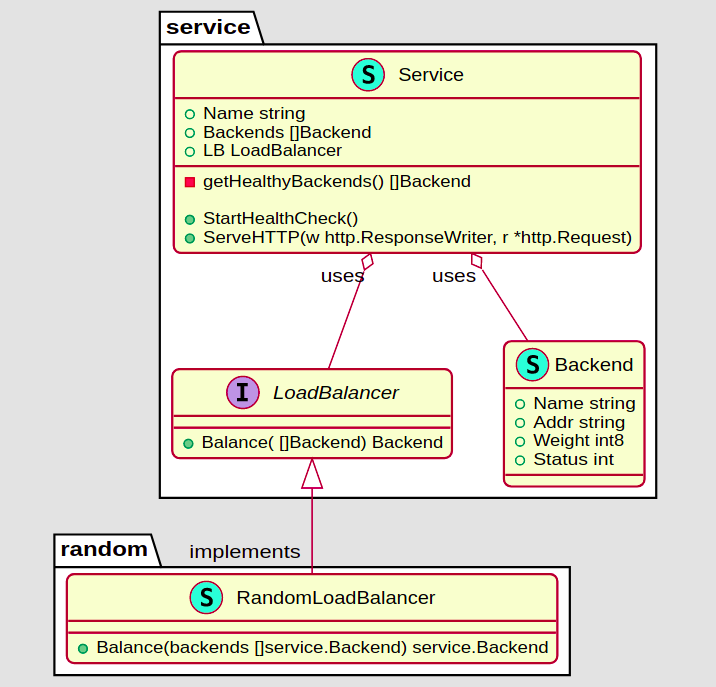
\includegraphics[scale=0.2]{images/Loadbalance.png}
\end{figure}

متعادل‌کننده‌های بار می‌توانند از وزن بطن‌های یک سرویس، برای توزیع وزن‌دار بار استفاده‌ کنند.


\subsubsection{تامین کننده‌ی خدمت‌ها}
تامین‌کننده‌ وظیفه تامین پیکربندی‌ خدمت‌های مختلف را دارد. با توجه به تنوع در محیط‌های بارگذاری سامانه‌های با معماری میکروسرویس، درگاه ارتباط باید بتواند با اجزاهای محیطی مختلف ارتباط برقرار کرده و تنظیمات مربوط به خدمت‌های مختلف را از این محیط‌ها دریافت کند. قطعه کد زیر نشان‌دهنده‌ی واسط مربوط به تامین کننده‌ی خدمت است.

\begin{latin}
    \begin{lstlisting}
                                    type ServiceProvider interface {
                                        Provide() ([]service.Service, error)
                                        Watch(messageChan chan<- Message) error
                                    }
    \end{lstlisting}
\end{latin}

تامین‌کننده به صورت یک واسط تعریف شده است و نسخه‌های پیاده‌سازی شده‌ی مختلف ‌آن‌ها، پیکربندی‌های مختلف را از محیط‌های متفاوت مانند \lr{Docker}، ‌\lr{Kubernetes} و ... جمع‌آوری می‌کنند.

شکل
\ref{provider}
نشان‌دهنده‌ی نمودار UML و نسخه‌های پیاده‌سازی شده از تامین‌کننده‌ی خدمت‌هاست.

\begin{figure}[H]
    \centering
    \caption{نمودار UML بسته‌ی Provider}
    \label{provider}
    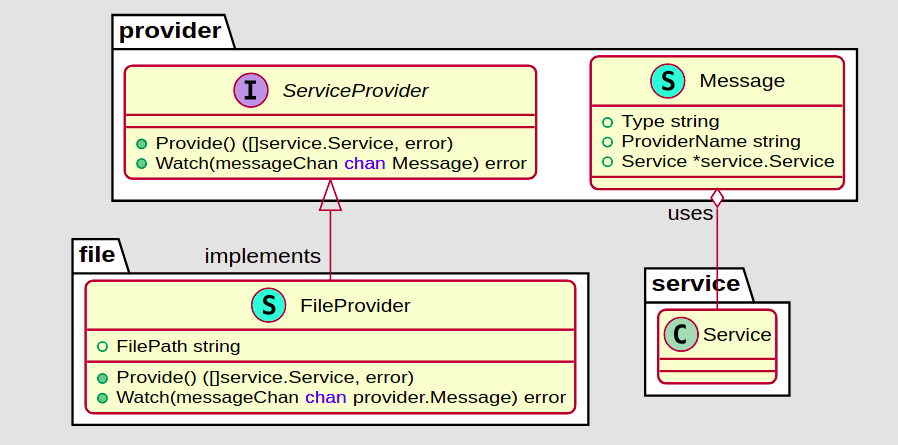
\includegraphics[scale=0.2]{images/Provider.png}
\end{figure}

\subsubsection{ضابطه}
ضابطه‌ها داده‌ساختار‌هایی هستند که می‌توان از طریق آن‌ها به خدمات دسترسی پیدا کرد. در قالب این گزارش، ضابطه‌ها تنها برای پروتکل‌های HTTP و HTTPS طراحی شده‌اند. با توجه به ویژگی‌های این پروتکل‌ها، ضابطه‌های مختلفی می‌توان تعریف کرد. برخی از این ویژگی‌ها عبارتند از:

\begin{itemize}
    \item نوع پروتکل (\lr{HTTP} یا \lr{HTTPS})
    \item مسیر درخواست \LTRfootnote{Path}
    \item آدرس میزبان درخواست \LTRfootnote{Host}
    \item نوع درخواست \LTRfootnote{Request Method}
    \item سرتیتر‌های درخواست \LTRfootnote{Headers}
    \item مولفه‌های پرس‌و‌جوی درخواست \LTRfootnote{Query Params}
    \item میان‌افزار‌ها
\end{itemize}

کاربرد و نحوه‌ی استفاده از میان‌افزار ها در قسمت
\ref{subsubsec:impl_middleware}
بررسی خواهد شد.


قطعه کد زیر، نمایان‌گر داده‌ساختار یک ضابطه است.

\begin{latin}
    \begin{lstlisting}
                                    type Rule struct {
                                        Service     *service.Service
                                        Schema      string
                                        PathPrefix  string
                                        Hosts       []string
                                        Methods     []string
                                        Headers     map[string]string
                                        Queries     map[string]string
                                        Middlewares []middlewares.Middleware
                                        handler     http.HandlerFunc
                                    }
    \end{lstlisting}
\end{latin}

\subsubsection{میان‌افزار}\label{subsubsec:impl_middleware}
گاهی نیاز است قبل از رسیدن درخواست به خدمت، تغییراتی در درخواست ایجاد شود. و یا برخی از سیاست‌های کنترلی مانند احراز هویت و تایید دسترسی قبل از رسیدن درخواست به خدمت بررسی شود.

در برخی از مواقع نیز این نیاز مطرح است که از نتایج درخواست‌ها مطلع شد و از آن‌ها برای تولید گزارشات و تهیه‌ی داده‌های آماری استفاده کرد.

میان‌افزار‌ها این نیاز‌ها را برطرف خواهند کرد. میان‌افزار‌ها نیز به صورت یک واسط تعریف شده‌اند و نسخه‌های پیاده‌سازی شده‌ی مختلف ‌آن‌ها نیاز‌های مختلف را رفع خواهند کرد. برنامه‌ی زیر نشان‌دهنده‌ی شمای این واسط است.

\begin{latin}
    \begin{lstlisting}
                        type Middleware interface {
                            Process(handler http.HandlerFunc) http.HandlerFunc
                        }
    \end{lstlisting}
\end{latin}

در سامانه‌ی پیاده‌سازی شده، میان‌افزار ها دو قسم اند. برخی از آن‌ها،‌که معمولا جز میان‌افزار‌های پرطرفدار در صنعت هستند، به صورت پیشفرض پیاده‌سازی شده‌اند.
میان‌افزار‌های از پیش آماده در این سامانه عبارتند از:

\begin{itemize}
    \item میان‌افزار CORS
    \item میان‌افزار محدود‌کننده‌ی نرخ درخواست \LTRfootnote{Rate limiter}
    \item میان‌افزار رصد سامانه
\end{itemize}

محدود‌کننده‌ی نرخ درخواست با استفاده از الگوریتم \lr{Token Bucket}
\cite{tokenbucket}
باعث می‌شود بتوان نرخ ارسال درخواست‌های کاربران را تحت کنترل قرار داد.

میان‌افزار CORS
\cite{cors}
نیز با استفاده از استاندارد‌های تعیین‌شده برای درخواست‌های با مبدا و مقصد مختلف، دسترس‌پذیری این سامانه‌ را از منابع مختلف تعیین می‌کند.

میان‌افزار رصد سامانه نیز، طبق استاندارد‌های نرم‌افزار \lr{Prometheus}،
\cite{prometheus}
امکان بررسی و تحلیل اطلاعات را فراهم می‌کند.

گروهی دیگر از میان‌افزار‌ها نیز توسط کاربران سامانه تعریف و پیاده‌سازی شده و به داخل سامانه تزریق می‌شوند. این ویژگی باعث می‌شود استفاده کنندگان از این سامانه، هیچ‌گونه وابستگی به توسعه‌دهندگان اصلی برنامه نداشته باشند و میان‌افزار‌های مربوط‌ به نیازمندی‌های خاص خود را پیاده‌سازی کرده و در سامانه تزریق کنند.

شکل
\ref{middlewares_package}
نشان‌دهنده‌ی نحوه‌ی پیاده‌سازی میان‌افزار‌ها با استفاده از واسط تعیین‌شده است.

\begin{figure}[H]
    \centering
    \caption{نمودار UML بسته‌ی Middleware}
    \label{middlewares_package}
    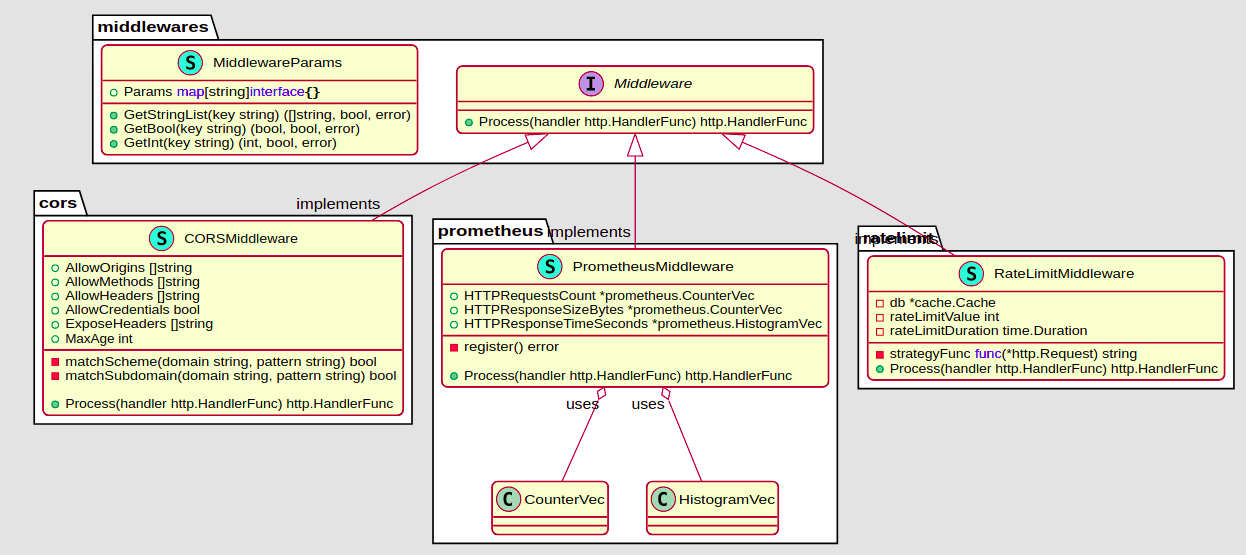
\includegraphics[scale=0.2]{images/Middleware.png}
\end{figure}

\subsubsection{مسیریاب}\label{subsec:impl_router}
یک درگاه ارتباط با رابط‌های برنامه‌نویسی را می‌توان یک مسیریاب لایه‌ی هفتم شبکه در نظر گرفت. بدین صورت که درخواست‌های ارسالی از سمت کاربران را به پاسخ‌دهنده‌های مربوط به آن‌ درخواست‌ها هدایت می‌کند.

یک مسیریاب به طور واسط تعریف شده‌ است و رفتار‌های مورد نیاز آن، بدون توجه به منطق پیاده‌سازی آن مشخص شده است. برنامه‌ی زیر تعریف یک واسط مسیریاب را نشان می‌دهد.

\cleardoublepage

\begin{latin}
    \begin{lstlisting}
                            type Router interface {
                                AddRule(rule rules.Rule) error
                                ServeHTTP(w http.ResponseWriter, req *http.Request)
                            }
    \end{lstlisting}
\end{latin}

مسیریاب‌ها با استفاده از ضابطه‌های تعریف‌شده، هر درخواست را به خدمت مورد نظر هدایت می‌کنند.

شکل
\ref{router_package}
نشان‌دهنده‌ی نحوه‌ی پیاده‌سازی یک مسیریاب با استفاده ‌از واسط تعیین شده است.

\begin{figure}[H]
    \centering
    \caption{نمودار UML بسته‌ی Router}
    \label{router_package}
    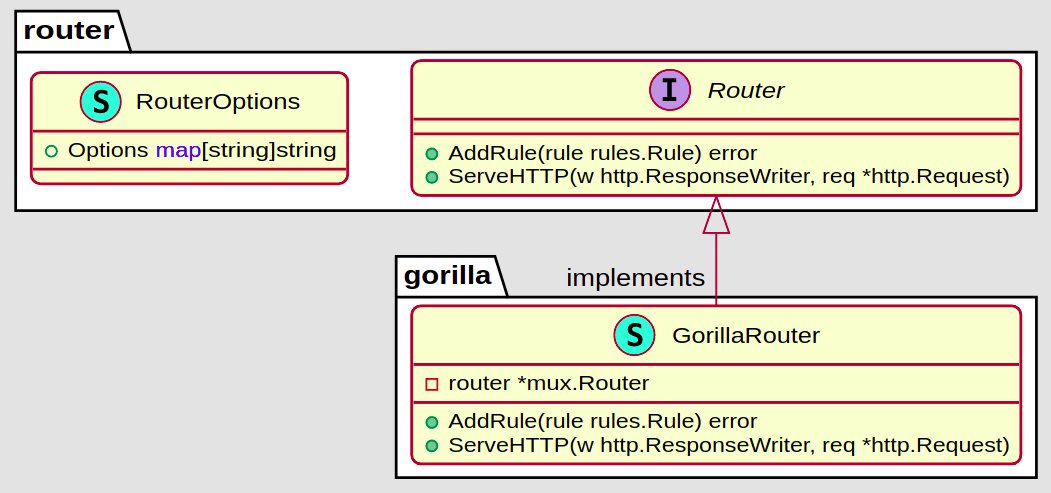
\includegraphics[scale=0.2]{images/Router.png}
\end{figure}

به طور کلی، شکل
\ref{flow}
نشان‌دهنده‌ی روند طی‌شده برای درخواست کاربران را به طور خلاصه شرح می‌دهد.

\begin{figure}[H]
    \centering
    \caption{روند طی‌شده برای هر درخواست}
    \label{flow}
    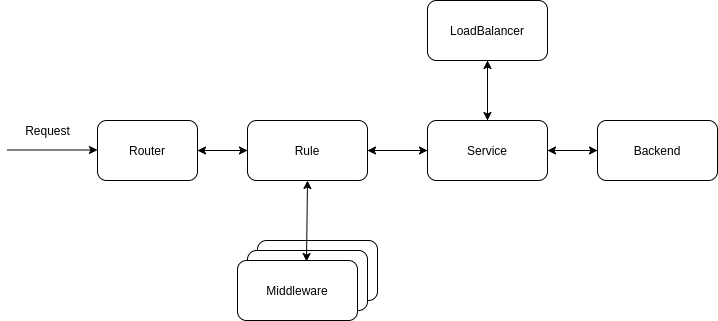
\includegraphics[scale=0.4]{images/Flow.png}
\end{figure}

\subsection{ویژگی‌های سامانه}\label{subsec:impl_features}
معماری ذکر‌شده در بخش
\ref{subsec:impl_concepts}
، ویژگی‌های زیر را داراست:

\begin{itemize}
    \item کمترین وابستگی ممکن
    \item آزمون پذیری بالا
    \item گسترش پذیری بالا
    \item مقیاس‌مندی بالا
\end{itemize}

\subsubsection{وابستگی}
با استفاده درست از واسط‌ها و همچنین طراحی ماژولار، بخش‌های مختلف سامانه کمترین وابستگی به یکدیگر را دارند. این ویژگی باعث می‌شود تغییرات احتمالی در آینده به راحتی هرچه تمام‌تر انجام شود.

\subsubsection{آزمون‌پذیری}
با توجه به وابستگی کم اجزای سامانه به یکدیگر،‌هر یک از اجزا می‌توانند به تنهایی مورد آزمون و ارزیابی قرار گیرند.
هم‌چنین استفاده از واسط‌ها امکان ایستا کردن یک بخش و انجام آزمون واحد
\LTRfootnote{Unit test}
بر روی بخش دیگر را امکان‌پذیر می‌کند.

\subsubsection{گسترش‌پذیری}
با توجه به استفاده به موقع از واسط‌ها، گسترش سامانه،‌ از طریق پیاده‌سازی نسخه‌های جدید از واسط‌ها، بسیار ساده خواهد بود. همچنین امکان تزریق میان‌افزار‌های پیاده‌سازی شده توسط کاربران استفاده کننده، بدون نیاز به کامپایل مجدد نرم‌افزار، خاصیت گسترش پذیری نرم‌افزار را افزایش می‌دهد.

\subsubsection{مقیاس‌مندی}
با توجه به عدم ذخیره‌ی حالت در سامانه، می‌توان تعداد نسخه‌های در حال اجرای سامانه‌ را به طور خطی برای افزایش میزان توان عملیاتی سامانه، زیاد کرد.

\cleardoublepage 